%!TEX root = Slic3r-Manual.tex
\section{Mati\`ere de Support} % (fold)
\label{sec:support}
\index{support material}
\index{mati\`ere de support}

En g\'en\'eral, la plupart des mod\`eles 3D seront imprim\'ees avec des parties en surplomb jusqu'\`a une certaine inclinaison. L'angle est d\'etermin\'e par plusieurs facteurs, notamment la hauteur de la couche et la largeur d'extrusion, et est g\'en\'eralement autour de 45 °. Pour les mod\`eles avec de plus grands surplombs une structure de support peut \^etre imprim\'e en dessous. Cela engage l'utilisation de plus de mati\`ere, plus le temps d'impression, et un nettoyage apr\`es l'impression.

\begin{figure}[H]
\centering
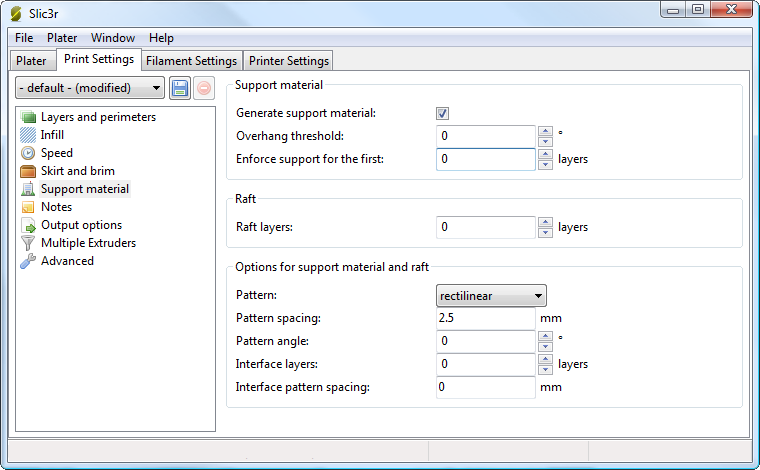
\includegraphics[keepaspectratio=true,width=1\textwidth]{expertmode/support/advanced_support.png}
\caption{Param\`etres de support.}
\label{fig:advanced_support}
\end{figure}
\index{Print Settings!Support material!Generate support material}
\index{Param\`etres d'Impression!Mati\`ere de Support!G\'en\'erer un support}
\index{Print Settings!Support material!Overhang threshold}
\index{Param\`etres d'Impression!Mati\`ere de Support!Seuil de porte \`a faux}
\index{Print Settings!Support material!Enforce support}
\index{Param\`etres d'Impression!Mati\`ere de Support!Appliquer le support}

La premi\`ere chose \`a faire est d'activer l'option de mati\`ere de support en cochant la case \texttt{Generate support material} (G\'en\'erer un support).  Mettre \`a z\'ero le param\`etre \texttt{Overhang threshold} (Seuil de porte \`a faux) indique \`a Slic3r de d\'etecter les lieux o\`u apporter un soutien automatiquement, sinon l'angle indiqu\'e sera utilis\'e.  La g\'en\'eration de support est un sujet relativement complexe, et il ya plusieurs aspects qui d\'eterminent le soutien optimal, il est fortement recommand\'e de fixer le seuil \`a z\'ero et permettre Slic3r de d\'eterminer le soutien n\'ecessaire.

Les petits mod\`eles, et ceux avec de petites empreintes \`a la base, peuvent parfois se briser ou se d\'etacher du lit.  Pour cette raison le param\`etre \texttt{Enforce support} (Appliquer le support) produira des structures de support \`a imprimer pour le nombre donn\'e de couches, ind\'ependamment de la valeur de seuil d'angle.

Pour d\'emontrer les modes de remplissage le mod\`ele minimug a \'et\'e inclin\'e de 45 ° le long de l'axe x, comme repr\'esent\'e sur la figure \ref{fig:support_minimug_45deg}.
\index{Print Settings!Support material!Pattern}
\index{Param\`etres d'Impression!Mati\`ere de Support!Motif}

\begin{figure}[H]
\centering
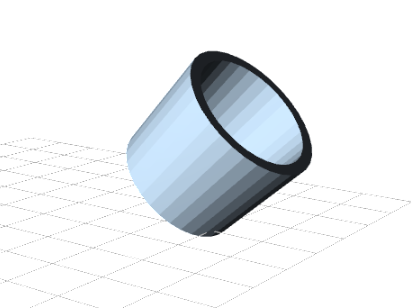
\includegraphics[keepaspectratio=true,width=0.75\textwidth]{expertmode/support/support_minimug_45deg.png}
\caption{Mod\`ele Minimug, inclin\'e \`a 45°.}
\label{fig:support_minimug_45deg}
\end{figure}

Comme avec le remplissage, il existe plusieurs motifs disponibles pour la structure de support.

\begin{figure}[H]
\centering
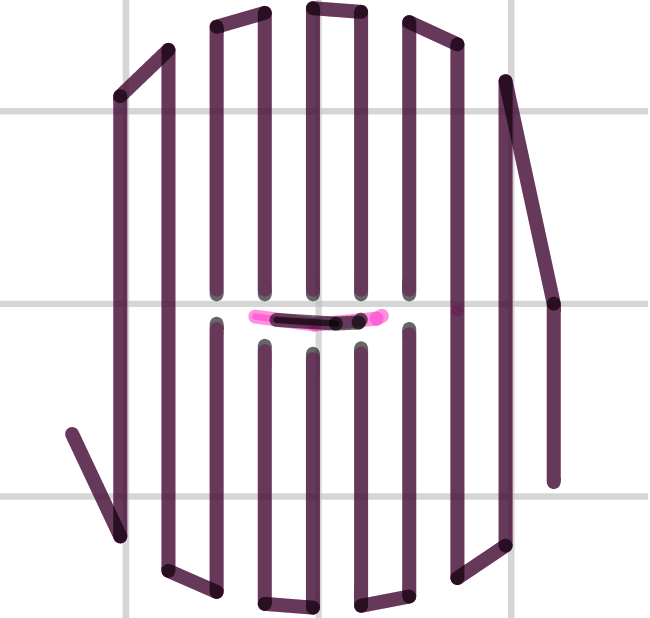
\includegraphics[keepaspectratio=true,width=0.2\textwidth]{expertmode/support/support_pattern_rectlinear.png}
\caption{Motif de support: Rectiligne}
\label{fig:support_pattern_rectlinear}
\end{figure}

\begin{figure}[H]
\centering
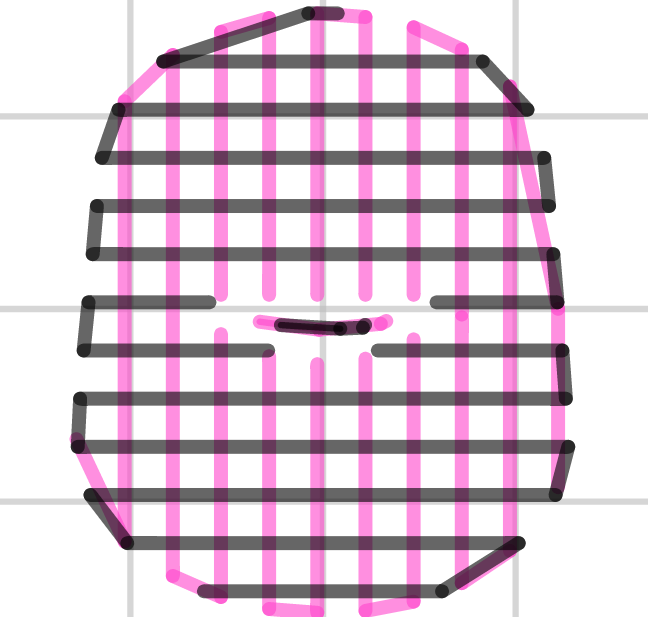
\includegraphics[keepaspectratio=true,width=0.2\textwidth]{expertmode/support/support_pattern_rectlinear_grid.png}
\caption{Motif de support: Grille Rectiligne}
\label{fig:support_pattern_rectlinear_grid}
\end{figure}

\begin{figure}[H]
\centering
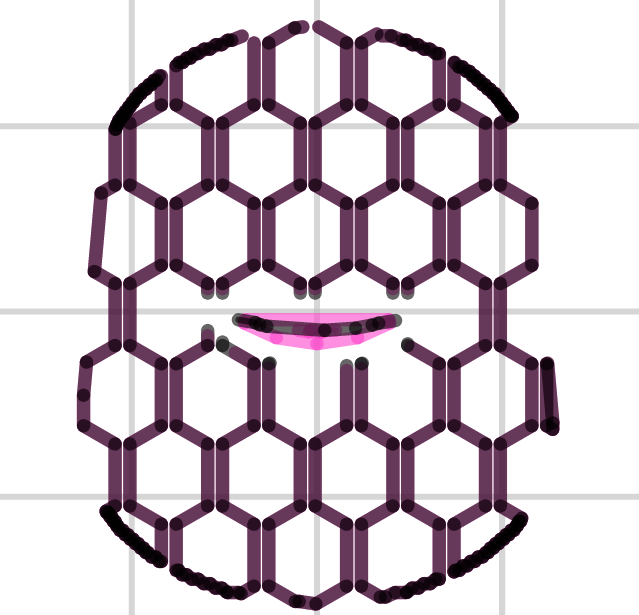
\includegraphics[keepaspectratio=true,width=0.2\textwidth]{expertmode/support/support_pattern_honeycomb.png}
\caption{Motif de support: Nid d'Abeille}
\label{fig:support_pattern_honeycomb}
\end{figure}
\index{Print Settings!Support material!Pattern Spacing}
\index{Param\`etres d'Impression!Mati\`ere de Support!Espacement du Motif}

\index{Print Settings!Support material!Pattern Angle}
\index{Param\`etres d'Impression!Mati\`ere de Support!Angle du Motif}

\texttt{Pattern Spacing} (Espacement du Motif) d\'etermine la distance entre les lignes de support, et est comparable \`a la densit\'e de remplissage en plus d'\^etre d\'efinie seulement en mm. Si vous changez cet attribut tenez compte de la largeur de l'extrusion du support et de la quantit\'e de mati\`ere de support qui adh\`ere \`a l'objet.

Il faut prendre soin de choisir un motif de support qui correspond au mod\`ele, o\`u le support se fixe perpendiculairement \`a la paroi de l'objet, plut\^ot que parall\`element, de sorte qu'il sera facile \`a retirer.  Si la structure de support court le long de la longueur d'une paroi alors le param\`etre \texttt{Pattern Angle} (Angle du Motif) permet la rotation de la direction des lignes de support

\begin{figure}[H]
\centering
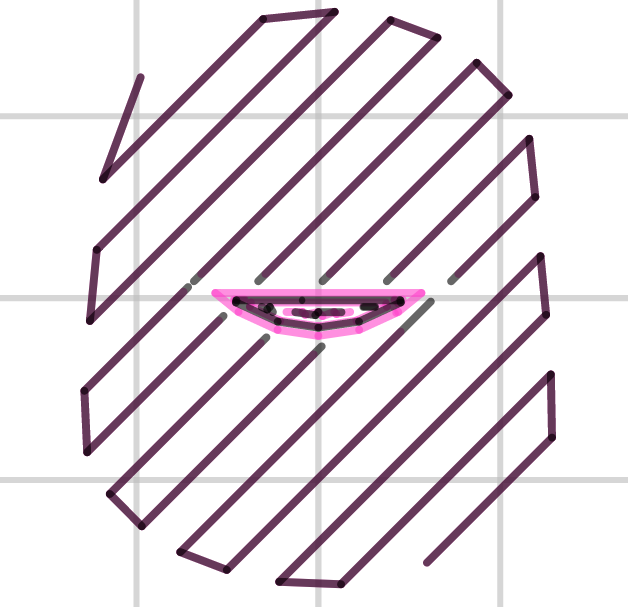
\includegraphics[keepaspectratio=true,width=0.2\textwidth]{expertmode/support/support_pattern_rectlinear_rotated.png}
\caption{Example de motif tourn\'e \`a 45°.}
\label{fig:support_pattern_rectlinear_rotated}
\end{figure}


%TODO: Interface layers.


% section support (end)